\chapter{Data}
\label{ch_data}






\section{ALMA Observations}
IRS 63 was observed in full polarization by ALMA at \bfour (Band 4), \bfive (Band 5), \bsix (Band 6), and \bseven (Band 7) between 2017-2022 \SCC{add project ID}. The \bandfivemm polarization observations were originally presented in \cite{sadavoy_dust_2019}, and the remaining datasets were presented in \cite{tobin} as continuum only. Information about the observations are outlined in Table \ref{tab: alma_observations}.



% Calibrator info was taken from shamus' thesis 
\begin{table}[h!]
\centering
\caption{ALMA Observation Information. \note{\cite{Tobin2024} also has 2017-05-13 and 2017-05-15 for observing dates for Band 6.} \note{\cite{Tobin2024} has number of antenna as 46, 45, 57, 42. also time of source as 8.06 for Band 6} \note{\cite{Tobin2024} has time of source as 8.06 for Band 6 and Sarah commented maybe 7.3 min}}
\begin{tabular}{lllll}
\toprule
\textbf{Property} & \textbf{\bandfourmm} & \textbf{\bandfivemm } & \textbf{\bandsixmm } & \textbf{\bandsevenmm} \\
\midrule

% Observed from
Observation Date
& 2019-09-01 % Band 4
& 2022-08-10 % Band 5
& 2017-05-20 % Band 6
& 2022-08-21 % Band 7
\\



& 2019-09-02 % Band 4
& ... % Band 5
& 2017-07-11 % Band 6
& ... % Band 7
\\


& ... % Band 4
& ... % Band 5
& 2017-07-14 % Band 6
& ... % Band 7
\\




$\nu$ (GHz) 
& 145 % Band 4
& 203 % Band 5
& 233 % Band 6
& 344 % Band 7
\\


Phase Calibrator
& J1633-2557 % Band 4
& J1617-2537 % Band 5
& J1625-2527 % Band 6
& J1626-2951 % Band 7
\\


Flux/Bandpass Calibrator
& J1517-2422 % Band 4
& J1517-2422 % Band 5
& J1517-2422  % Band 6
& J1517-2422 % Band 7
\\


Polarization Calibrator
& J1751+0939 % Band 4
& J1751+0939 % Band 5
& J1549+0237 % Band 6
& J1751+0939 % Band 7
\\



Time on Source (min)
& 37.7 % Band 4
& 35.62 % Band 5
& $\approx$ 7 % Band 6
& 30.81 % Band 7
\\



Min. Baseline (m)
& 38 % Band 4
& 15 % Band 5
& 15 % Band 6
& 15 % Band 7
\\


Max. Baseline (m)
& 3638 % Band 4 (3637.743277)
& 1302 % Band 5 (1301.611)
& 2647.3 % Band 6
& 1302 % Band 7 (1301.611)
\\



% Antennas:
\# Antenna
& 47 % Band 4
& 45 % Band 5
& 42-46 % Band 6
& 45 % Band 7
\\






% Pixel ($''$) 
% & 0.018 
% & 0.018 
% & 0.018 
% & 0.018 \\


\bottomrule
\end{tabular}
\label{tab: alma_observations}
\end{table}








% \begin{table}[h!]
% \centering
% \caption{\add{Caption}}
% \begin{tabular}{cccccc}
% \toprule
% \multirow{2}{*}{} & \multicolumn{2}{c}{\textbf{Center position (J2000)}}  & \textbf{Disk PA}  \\
% & R.A. (h, m, s) & Decl. ($^\circ$,$'$,$''$)  & ($^\circ$)  \\
% \midrule 
% \textbf{Band 4} & 16:31:35.656 & -24:01:29.992 & 145.9  \\
% \textbf{Band 5} & 16:31:35.656 & -24:01:30.086   & 140.25 (check)   \\
% \textbf{Band 6} & 16:31:35.657 & -24:01:29.935  & 148.0   \\
% \textbf{Band 7} & 16:31:35.656 & -24:01:30.089  & 139.65  \\
% \bottomrule
% \end{tabular}
% \label{tab: source_info}
% \end{table}









\section{Self-Calibration}



% \draft{In the last chapter, we summarized how the visibilities were calibrated by ALMA before we recieved the data. Beause IRS 63 is a bright and nearby source the observations have a high SNR, sllowing us to do self-calibration. Self-calibration is useful to get rid of the `stuff' that pops up but is not really there, called an artifact \citep{Marvil2}. First, there could be artifacts from the srouce duue to calibration errors such as differences in the astmosphere over each dish \citep{Marvil2}. Secondly, there could be artifacts from a backgrournd source due to direction-independent calibration errors, such as antenna based gain changes \citep{Marvil2}.}


In this section, the self-calibration details for this project are summarized. The data at \bfourNS, \bfive and \bseven were calibrated as part of this project, and the \bsix data were provided from \cite{sadavoy_dust_2019}.


To clean the data,  \texttt{tclean} was used in Common Astronomy Software Applications (CASA) version 5.6.1-8 \SCC{add casa citation}. The images were cleaned using the multi-scale multi-frequency deconvolution algorithm (MS-MFS, \texttt{deconvolver = `mtmfs'}). Different values of nterms were explored and no significant change between \texttt{nterms = 1} and nterms = 2 were found. The images presented in this thesis have nterms = 2 for \bfour and \bsevenNS, nterms = 1 for \bfive and \bsixNS. 
\question{band 5 nterms = ?} The Briggs weighting scheme was used with \texttt{robust = 0.5} for all wavleengths except the \bfive data where w\texttt{robust = -1} was used to better match the resolution of the other datasets (see Chapter \ref{sec: discussion_band5_data_issues} for more details). 



The \SI images at each band had an interactive clean at both phase and amplitude calibration. We began with a shallow phase calibration, and progressively cleaned deeper each time for a total of three rounds. Then, two rounds of amplitude and phase self calibration. \SC{Add more info.} Additionally, the \SQ and \SU data were also cleaned using a non-interactive phase calibration using the final mask from the amplitude calibration at its respective wavelength.  \SC{Add more info}


Below, in Figure \ref{fig: BeforeAndAfterClean}, is an example of IRS 63 at \bfour before and after self calibration. We can see how cleaning the image removed background noise. The \SNR values also improved, going from 660 to 2655. \question{Report the S/N change for the other bands?}. The final self-calibrated \SI maps produced using this method are presented in Chapter \ref{sec: chap4_stokesI}.


\SC{It may be worth here or in the previous section to explain how self-calibration can improve the S/N.}



\begin{figure}[h]
  \centering
  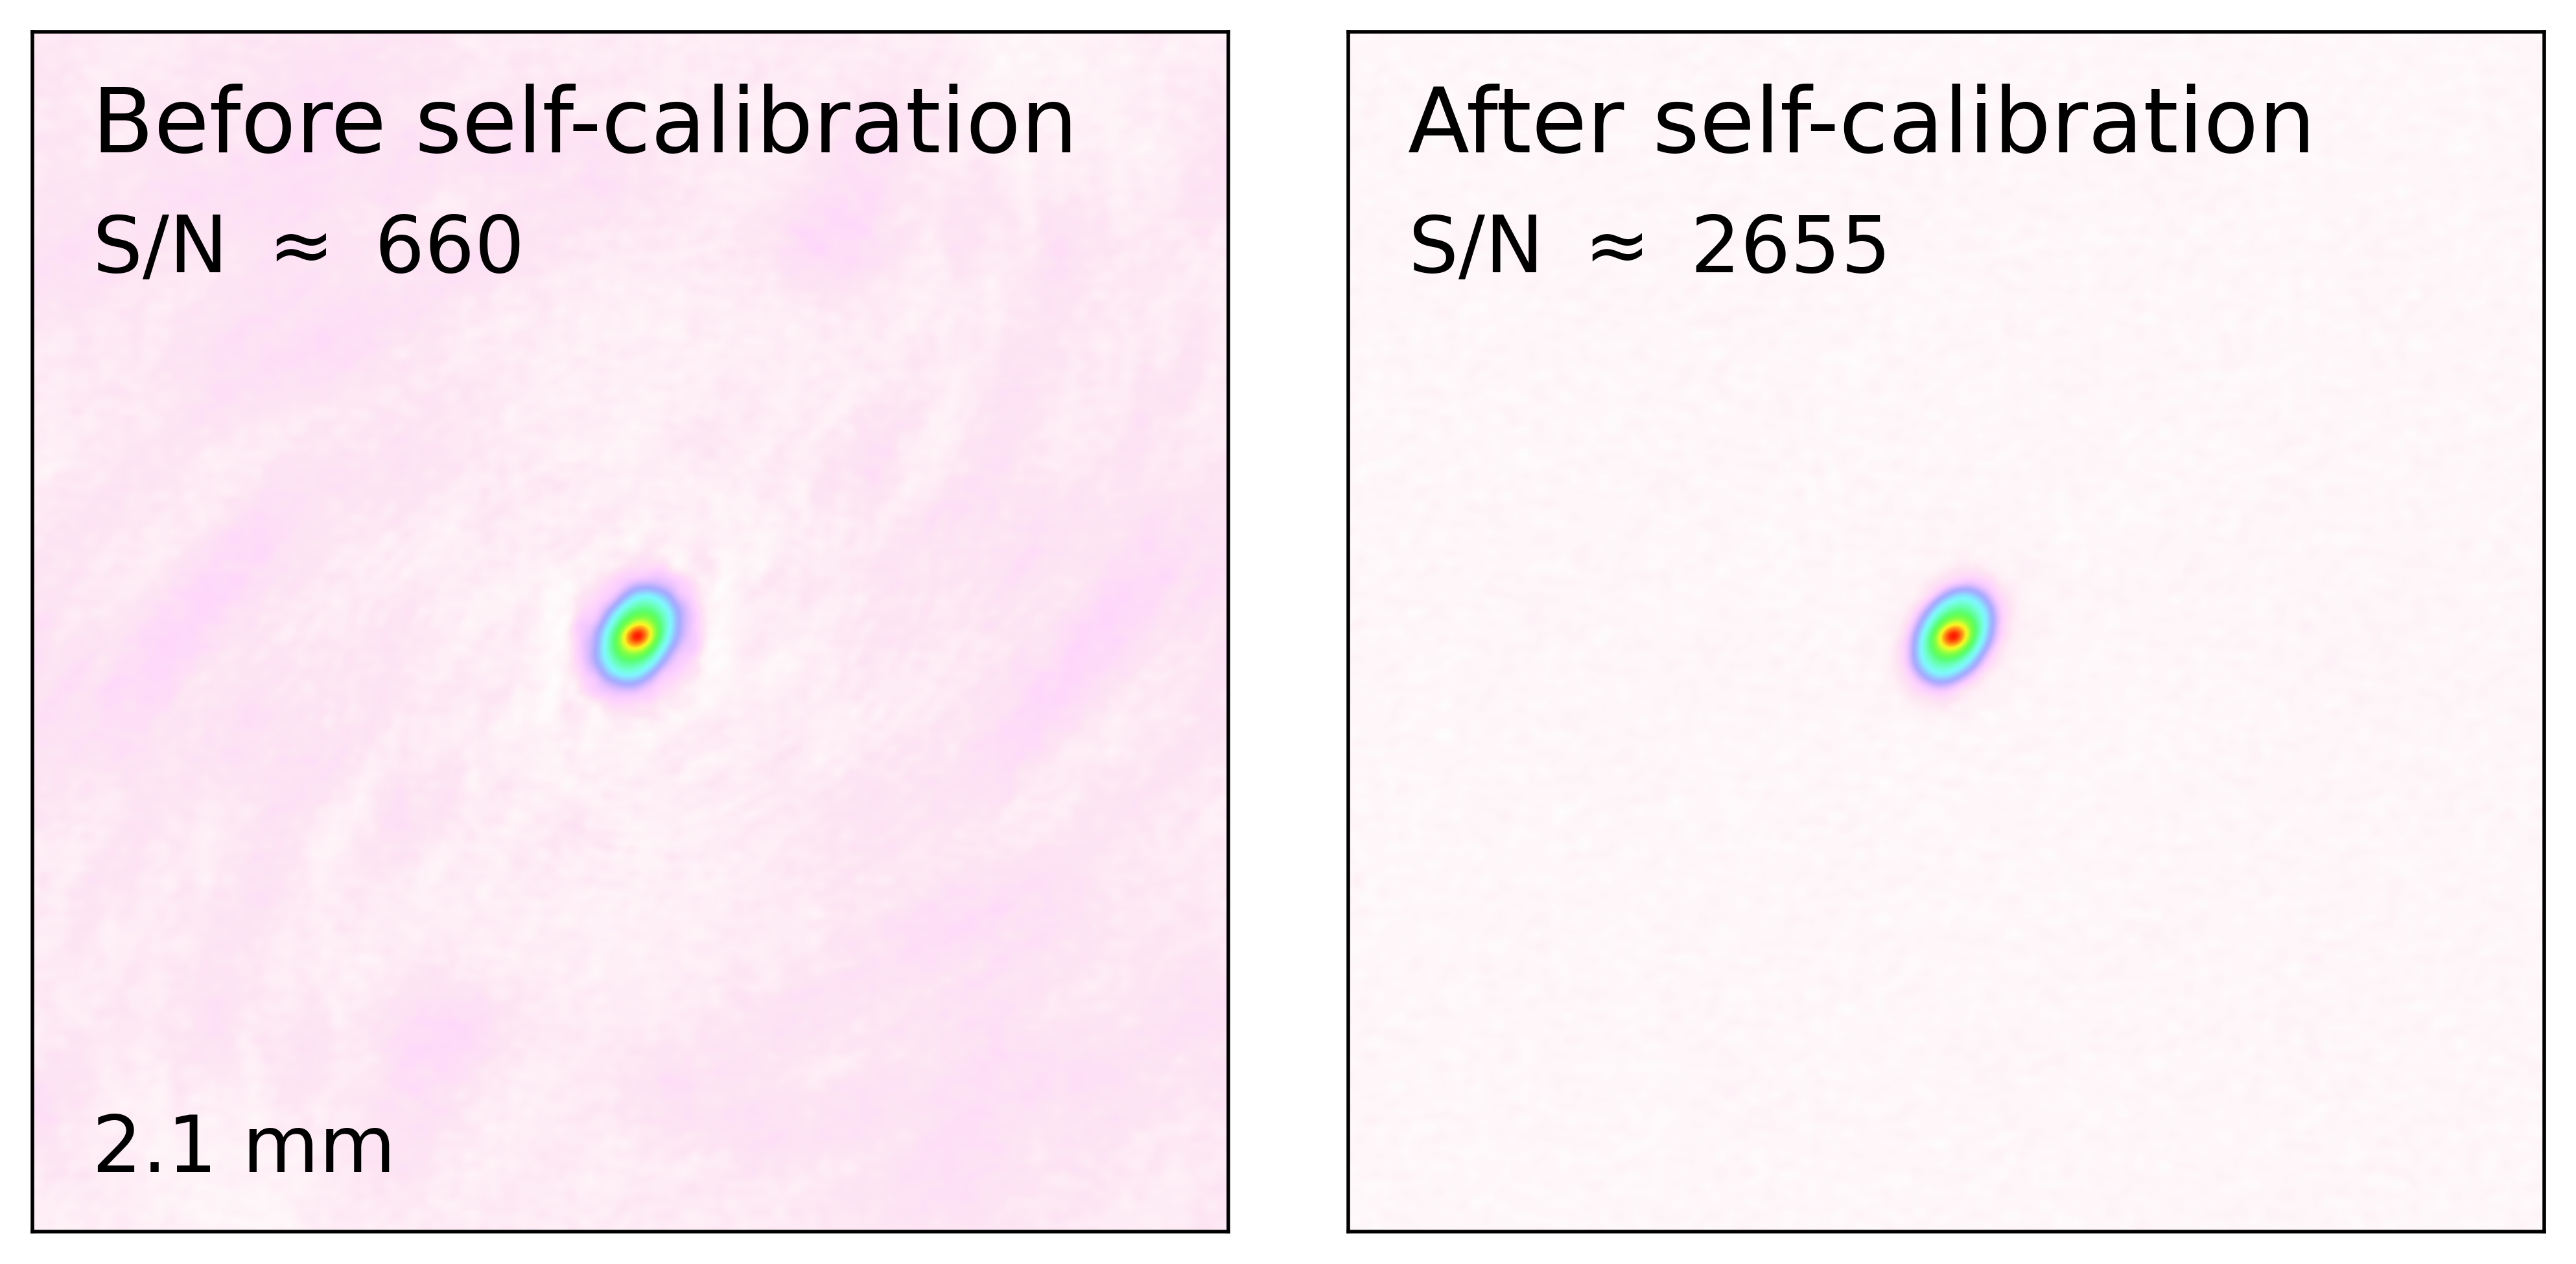
\includegraphics[width=1.25\textwidth]{WRITEUP_AND_IMAGES/IMAGES/WRITEUP/BeforeAndAfterClean.png}
  \caption{Images before (left) and after (right) self-calibration at \bfour. Images shown to demonstrate how background noise is reduced the self-calibration process, and improved the peak \SNRns.}
  \label{fig: BeforeAndAfterClean}
\end{figure}




\SCC{The results of the self-cleaning process are presented in Table \ref{tab: source_info}, including the synthesized beam size, reported as major and minor axes and position angle. } Additionally, the centre position of the disk in Right Ascension (RA) and Declination (Dec) and the position angle of the disk found using \SCC{\texttt{imfit} in CASA.}


\begin{table}[h!]
\centering
\caption{Summary of properties of the cleaned images of IRS 63. \add{Band 5 robust -1 not 0.5, nterms and robust}}
\begin{tabular}{lcccc}
\toprule
\textbf{Property} & \textbf{\bandfourmm} & \textbf{\bandfivemm } & \textbf{\bandsixmm } & \textbf{\bandsevenmm} \\
\midrule


R.A. (h, m, s) 
& 16:31:35.656 
& 16:31:35.656 \note{check}
& 16:31:35.657  
& 16:31:35.656 \\

Decl. (J2000) 
& -24:01:29.992 
& -24:01:30.086 \note{check}
& -24:01:29.935 
& -24:01:30.089 \\


Beam ($''\times''$) 
& 0.18 $\times$ 0.13 
& 0.23 $\times$ 0.18 
& 0.27 $\times$ 0.20 
& 0.28 $\times$ 0.17 \\



Beam PA ($^\circ$) 
& -81.0 
& -88.9 \add{$\Delta$ to rob-1}
& -68.6
& -81.2 \\


Disk PA ($^\circ$) 
& 145.9 
& 148.39 \note{check}
& 148.0 
& 139.7 \\

\texttt{nterms}
& \add{num}
& \add{num}
& \add{num} 
& \add{num} \\

\texttt{robust}
& \add{num}
& \add{num}
& \add{num} 
& \add{num} \\



\bottomrule
\end{tabular}
\label{tab: source_info}
\end{table}




% ---------------------------------------------





\section{Debias Correction}

\question{Call this unbiased or observed?}

The unbiased polarized intensity, \POLIobsNS, is calculated from \SQ ($Q$) and \SU ($U$) using the equation: 
\begin{equation}
    \POLIobsEQ = \sqrt{Q^2 + U^2}.
    \label{eq: POLI}
\end{equation}
\noindent Since \SQ and $U$ are squared, the equation always yields a positive value. This positive outcome produces a bias when either $Q$ or $U$ are dominated by noise. To account for this bias, a debiased polarized intensity is calculated. 
% noise gives us Q and U not equal to 0 even when it should be 0, more noise -> higher POLI value



The polarized intensity was de-biased using the method explained in \cite{sadavoy_dust_2019}, originally from \cite{HullDebias}, with equations from \cite{CoudeEquations}. This method calculated the debiased polarized intensity, \POLIns, with a corresponding error of \POLIerr with the equation:

\begin{equation}
    \text{PDF}(\POLIeq|\POLIobsEQ, \POLIerrEQ)=\frac{\POLIobsEQ}{\POLIerrEQ^2} I_0(x)\exp\left[-\frac{(\POLIobsEQ^2 + \POLIeq^2)}{2\POLIerrEQ^2}{}\right],
    \label{eq: debias}
\end{equation}
\noindent where PDF is the probability density function. Here, $I_0(x)$ is the Bessel function for the Bessel parameter $x = \POLIobsEQ \POLIeq/\POLIerrEQ^2$. The most likely \POLI will create a peak in Equation \ref{eq: debias}, so the debiased value is calculated by minimizing the negative value of the PDF in Equation \ref{eq: debias} using \texttt{scipy.optimize.minimize\_scalar}. Only the pixels with a S/N$<9$ were diabsed with this method. \question{add a sentence on why 9 was used? \SCC{A}} 

The pixels with S/N$>9$ do not need to be treated the same way since their emission is so bright, and are debiased using the standard maximum likelihood calculation method from \cite{VaillancourtDebias}:
\begin{equation}
   \POLIbrightEQ = \sqrt{Q^2 + U^2 -\POLIerrEQ^2}.
\end{equation}


\noindent The corresponding error of the debiased polarized intensity is calculated by:

\begin{equation}
    \POLIerrEQ = 
    \left[ 
    \frac{(Q\SQerrEQ)^2 + (U\SUerrEQ)^2}{Q^2 + U^2} \right]^{1/2}.
    \label{eq: PA_error}
\end{equation}









\section{Additional Polarization Quantities \& Errors}



% ---------------------------------------------
\subsection{Errors for Stokes Parameters}
\label{sec: stokes_errors}

For the data calibrated in this project (\bfourNS, \bfiveNS, \bsevenNS), the errors for \SIns, \SQ and \SU were estimated by averaging the maximum standard deviation in four different regions far from the bright source at the centre. This average value was applied as a constant error at every pixel in the respective error maps. Table \ref{tab: source_info} gives the errors at each wavelength. The errors for the \bsix data were estimated using the same method. 

% ---------------------------------------------
\subsection{Polarization Fraction and Angle}

The following equations in this Chapter are from \cite{CoudeEquations}, unless specified otherwise. 

Using the debiased polarized intensity, the debiased polarization fraction can be calculated by:
\begin{equation}
    \POLFeq = \POLIeq/I,
    \label{eq: POLF}
\end{equation}
\noindent where $I$ is \SI intensity. The uncertainty on polarization fraction is:

\begin{equation}
    \POLFerrEQ = \POLFeq \left[\left(\frac{\POLIerrEQ}{\POLIeq}\right)^2 + \left(\frac{\SIerrEQ}{I}\right)^2\right]^{1/2}.
     \label{eq: POLF_error}
\end{equation}
   


The polarization position angle, $\theta$ is calculated as: 
\begin{equation}
\theta = \half \tan ^{-1} \frac{U}{Q},
    \label{eq: PA}
\end{equation}
\noindent where $\theta$ has units of radians, and an uncertainty calculated by:

\begin{equation}
    \PAerrEQ = \frac{1}{2} 
    \frac{\sqrt{(U\SQerrEQ)^2 + (Q\SUerrEQ)^2}}{Q^2 + U^2}.
    \label{eq: PA_error}
\end{equation}
 

\noindent When measuring the angles, the zero-degree position is defined as North, with the polarization angle increasing counterclockwise from North to East. The coordinate system was previously shown in see Figure \ref{fig: LinearPol}. 



% ---------------------------------------------










